\subsubsection{Molecular Cell Biology - Biomedicine of Proteolysis}
\index{Brix, Klaudia}

\paragraph{Research Team}

Klaudia Brix (Professor), Heiko B�th (PhD completed in April 2006), Stefanie Dannenmann (Graduate Student), Anna Dunkhorst (PhD Student), Silvia Jordans (PhD completed in February 2006, Postdoctoral Fellow), Malgorzata Kubica (Visiting PhD Student), Kristina Mayer (PhD completed in January 2006, Postdoctoral Fellow), Hong Qu (PhD completed in May 2006), Maren Rehders / Meike Klepsch (Lab Technicians), Lakshmi Settu (Graduate Student), Ruxandra Sirbulescu (Graduate Student), Brit Wolters (PhD completed in March 2006)\\

Our research focus is to understand epithelial organs such as intestine, skin, and thyroid on the cellular and molecular level. As a biomedically-oriented group, our goal is to analyze the functions of these organs and to propose concepts, which might help in the development of novel therapeutic strategies. Our research is focused on proteolytic processes performed by lysosomal cysteine cathepsins. Using a combination of biochemical, cell and molecular biological research approaches, we analyze the spatio-temporal regulation of proteolysis and protease interaction in networks existing in defined biological systems of mammalian organisms. Thus, we get more insight into a general understanding of proteolytic processes in order to interfere with immobility of the gut with its most severe clinical complication of intestinal atony, scar formation as a result of improper wound healing of the skin, and dysfunction of the thyroid resulting in hormone deficits.

\paragraph{Highlights}
%
The main task of the thyroid gland is the production of thyroid hormones which are essential for brain development, growth, and regulation of metabolism and body temperature. Disorders of the thyroid are frequently observed. Hypothyroidism and goiter may arise as a result of iodine deficiency. In severe cases of low-iodine diets the phenotype of cretinism still occurs. We identified thyroglobulin, the precursor of thyroid hormones, as one of the natural  substrates of lysosomal cysteine peptidases. Through the use of cathepsin-deficient mouse models, we showed that the intra- and extracellular actions of cathepsins B, K, and L maintain thyroid function. Recently, we began to investigate the significance of cysteine cathepsin K for proper brain development in mouse models by combining behavioral studies with biochemical and cell biological approaches in order to explain the observed learning and memory phenotypes on the molecular level.

In cell-based assays, trafficking analyses were performed that comprised expression of GFP-tagged cathepsins with or without active-site-mutations, and cathepsin variants derived from tumor cells, as well as the use of activity-based probes to visualize transport and proteolytic activities of the enzymes in living cells. The results proved that the primary sequence and proper folding of the proteases is sufficient to correctly target cysteine cathepsins into endocytic compartments of normal epithelial cells. However, altered trafficking in carcinoma cells often results in mislocalization of cysteine cathepsins. Hence, cellular transport logistics do not depend on the cargo but rather on the cells themselves. This notion bears important implications for the molecular mechanisms underlying altered transport pathways of cysteine cathepsins in pathological conditions such as cancer.

During regeneration from wounding, secreted cathepsin B mediates keratinocyte migration for rapid wound closure by proteolysis and remodeling of the extracellular matrix. Specific receptors at the plasma membrane ensure restriction of the proteolytic activity of cathepsin B to the basal pole of the migratory cells. In contrast, trafficking of cathepsins L and V follows different routes in keratinocytes. Cathepsin L remains largely unaffected when human keratinocyte cell lines were wounded. However, a truncated version of cathepsin V is translocated to the nuclei of regenerating cells before keratinocytes start to proliferate. Future experiments aim to verify a causal relation between these two events and shall elucidate the molecular mechanisms that are initiated by the appearance of cathepsin V within the nuclei of keratinocytes.


\begin{figure}[ht]
  \begin{center}
   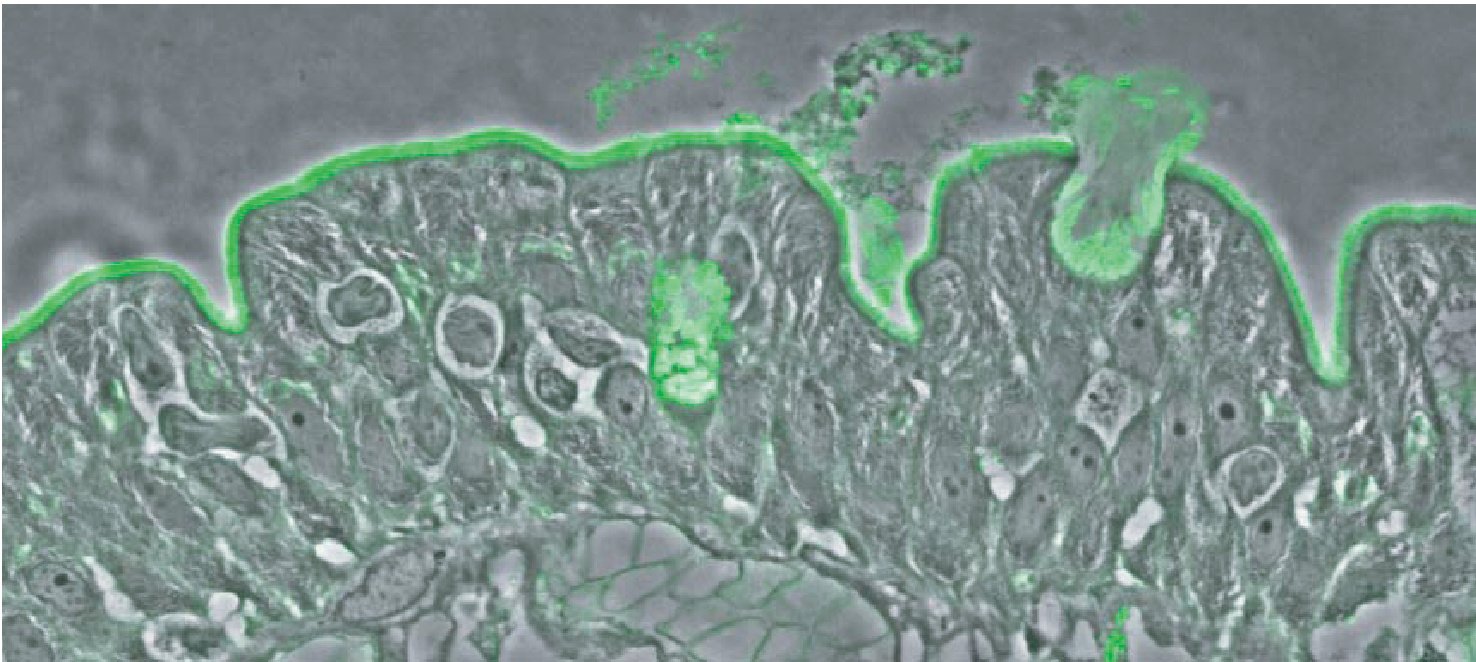
\includegraphics[width=\hsize]{Brix/Brix_2006_Fig.pdf}
    \mycaption{Cathepsin L expression in enterocytes and goblet cells of the mucosa of the small intestine; confocal laser scanning microsopy.}\label{fig:profBrix}
   \end{center}
\end{figure}


Recently, we hypothesized that non-regulated release of proteolytic enzymes as a result of tissue damage due to surgical trauma may have dramatic consequences for the affected tissue. Our studies on intestine trauma focus on the possible contribution of cathepsins to the onset of inflammatory responses, ultimately leading to dysfunction of intestinal smooth muscles and post-operative ileus, which is a severe and potentially life-threatening complication common in the clinics. Using standardized models of intestine trauma in mice and rats, we observed a local cathepsin B release concomitant with extracellular matrix damage during initial post-operative phases. Interestingly, cathepsin B-deficient animals showed an increased deposition of extracellular matrix components in the intestine. We concluded that the observed massive degradation of extracellular matrix in traumatized intestine might be a result of direct proteolytic action of released cysteine peptidases such as cathepsin B, or be driven by a more indirect activation of proteolytic cascades. As a possible consequence of the alterations of proteolytic activities due to trauma, impairment of the mucosal barrier function can occur, which will in turn severely affect homeostasis of the intestine. To assess the role of cathepsins during trauma at the molecular level, we established an \textit{in vitro} model that allows to simulate surgical trauma through mechanical compression of cultured intestinal epithelial cells. Finally and most recently, we established a transgenic mouse model with intestine-specific expression of GFP-tagged cathepsin B under the control of the A33-antigen promotor that now allows to directly investigate cysteine peptidase trafficking as well as its release and re-internalization pathways during the acute inflammatory phase and during regeneration from surgical trauma of the intestine.

In conclusion, analysis of trafficking, regulated secretion and non-regulated release of lysosomal cysteine cathepsins in combination with the identification of their natural substrate targets will help to better understand the biology of epithelial cells in physiological and pathological circumstances.


\paragraph{Organization}
\begin{enumerate}
\item 3rd Keratinocyte - Symposium / DFG-Forschergruppe ``Keratinocytes - Proliferation and Differentiation in the Epidermis''; Chair: V. Herzog; Organizing Committee: Th. Bieber, K. Brix, V. Herzog, Th. Magin, K. Sandhoff, Th. T�ting, K. Willecke. Uni-Club Bonn, Germany. April 27-28, 2006.
\item Poster Evaluation Committee Member of Gordon Research Conference ``Proprotein Processing, Trafficking and Secretion'', Chair: Nabil G. Seidah. Colby-Sawyer College, New London, NH, USA. July 9-14, 2006.
\item Scientific Advisory Committee Member in preparation of the 5th General Meeting of the International Proteolysis Society, Chair: Georgia Sotiropoulou, to be held in 2007 in Patras, Greece.
\item K. Brix was awarded Membership of the British Society for Matrix Biology.
\item K.Brix was appointed as Member of  the Organizing Committee of Gordon Research Conference ``Proprotein Processing, Trafficking and Secretion'', Chair: R.Mains, to be held in 2008 in New London, NM, USA.

\end{enumerate}

\myparagraph{Collaborations}
%
Bremen Area Collaborations:
\begin{enumerate}
\item {\sl International University Bremen} \\ Prof. A. Jeltsch \\ DNA Binding Proteins
 \\ Prof. K�hler\\ Thyroid Evolution / AWI
 \\ Dr. N. K�hl \\ Brain Proteases
 \\ Prof. A. Materny \\ Raman Spectroscopy of Cells
 \\ Prof. G. Muskhelishvili \\ DNA Binding Proteins
 \\ Prof. W. Nau \\ Dye Stabilization in Live Cells
 \\ Prof. M. Zacharias \\ Models for Protease Trafficking
\item {\sl AWI}\\ Dr. U. Passow \\ Exopolymers for Cell Culture
\end{enumerate}
National \& International Collaborations:
\begin{enumerate}\item {\sl Stanford University, School of Medicine, Stanford, USA} \\ Prof. M. Bogyo, Dr. G. Blum \\ Activity-based Probes for Visualization of Protease Activities
\item {\sl DKFZ, Heidelberg} \\ Prof. P. Boukamp \\ Migration of HaCaT Keratinocytes
\item {\sl University of British Columbia, Vancouver, Canada} \\ Prof. D. Broemme \\ Recombinant Cathepsins
\item {\sl University of Bonn} \\ Prof. J. Kalff, Dr. S. Wehner \\ Standardized Rat Intestine Trauma Model
\item {\sl University of Freiburg} \\ Prof. C. Peters, Dr. T. Reinheckel \\ Cathepsin B- and L- Deficient Mice
\item {\sl University of Mainz} \\ Prof. C. Pietrzik \\ LDL-Receptor Related Protein-1
\item {\sl University of Kiel} \\ Prof. P. Saftig \\ Cathepsin K-Deficient Mice
\item {\sl Wayne State University, Detroit, USA} \\ Prof. B. Sloane \\ Tumor Cell-Derived Cathepsin B
\item {\sl Jozef-Stefan Institute, Ljubljana, Slovenia} \\ Prof. B. Turk, Dr. N. Kopitar-Jerala \\ Cathepsin L and V Antibodies
\item {\sl University of Halle} \\ Dr. E. Weber \\ Cathepsin L and V Antibodies
\item {\sl University of Bielefeld} \\ Dr. N. Schaschke \\ Cathepsin B Inhibitors
\item {\sl University of Freiburg} \\ Dr. T. G�nther, Dr. T. Reinheckel, Prof. R. Sch�le  \\ Transgenic Mouse with Intestine-Specific Expression of Cathepsin B-GFP
\item {\sl Jagiellonian University, Krakow, Poland} \\ Prof. J. Potempa, M. Kubica (EMBO Shortterm-Fellow Exchange Student)\\ Cellular Compartments Hosting Infections Bacteria
\item {\sl The Centenary Institute, Cancer Medicine and Cell Biology, Sydney, Australia} \\ Prof. M. Gorrell \\ DPP IV
\item {\sl Uppsala University, Department of Genetics and Pathology, Uppsala, Sweden} \\ Prof. N.-E. Heldin \\ Thyroid Carcinoma Cell Lines
\item {\sl Triple Point Biologics, Forest Grove, OR, USA} \\ Dr. P. Alexander \\  Thyroid Antigen
\item {\sl University of British Columbia, Vancouver, Canada} \\ Dr. R. Kappelhoff, Prof. C.M. Overall \\ CLIP-Chip
\item {\sl Monash University Melbourne, Department of Biochemistry and Molecular Biology, Melbourne, Australia} \\ Prof. P. Bird, Prof. R. Pike, Prof. J. Whisstock \\ Serpins
\end{enumerate}


\paragraph{Grants}
\begin{enumerate}
\item Funded by DFG, \emph{Funktion von Cysteinproteasen f�r die
Migration und Differenzierung von Keratinocyten in der
Regenerationsphase nach Verletzung der Haut, BR 1308/6-1 and 6-2.
This project is performed in collaboration with the Forschergruppe
(FOR 367) ``Keratinocyten - Proliferation und differenzierte
Leistung in der Epidermis''.}, (March 2003 - March 2006)  \\

\item  Funded by DFG, \emph{Extrazellul�re Proteolyse nach
operativer Sch�digung des Darmepithels, BR 1308/7-1, 7-2, and 7-3.
This project is performed in collaboration with the Klinische
Forschergruppe (KFO 115) ``Molekulare und zellul�re Grundlagen der
intestinalen postoperativen Pathophysiologie''.}, (February 2003 -
March 2006 (BR 1308/7-1, 7-2),  February 2006 - January 2009 (BR
1308/7-3)
\end{enumerate}


\paragraph{Awards, Prizes}
\begin{enumerate}
\item   S. Jordans received the Poster Award and the Presentation Award at BSMB-Meeting on ``Proteases - the cutting edge of cell biology'', Chair: Graham Riley, Queen's College, Cambridge, UK.
\end{enumerate}

\nocite{Brix1,Brix2}
